Für diese Referenzarchitektur käme sowohl der Dienst der Multimode Klasse, \AWSIOT{} Analytics, als auch Timestream, als bester der Batch-Klasse in Frage. Da Timestream im Vergleich besser abschnitt, wird im Folgenden die Referenzarchitektur mit Timestream konstruiert.
Diese Referenzarchitektur entspricht dem in \autoref{chap:bestehende_ras} vorgestellten Konzept einer \ac{OLAP}-Architektur. Folgend wird auf die verschiedenen Dekompositionen inklusiver mit der Echtzeitreferenzarchitektur gemeinsamen Variationspunkte (\textbf{VP GX}) eingegangen.

\subsection{Datenverarbeitungssequenz}
In \autoref{abb:SequenceBatchRA} ist die Datenverarbeitungssequenz der Referenzarchitektur zu sehen. Die Daten werden mittels einer properitären Verbindung von \AWSIOT{} Core an Timestream überspielt und von Timestream gespeichert. In einem regelmäßigen Intervall (ähnlich zu den \textit{cron-jobs} auf Linux) wird eine Lambda Funktion aufgerufen. Diese fragt Timestream ab, interpretiert die Resultate und löst im Alarmfall Nachrichten an \ac{SNS} aus. QuickSight greift als Visualisierungslösung, wenn gewünscht, auf den gesamten Datenbestand von Timestream zu. Dies passiert entweder beim Abruf von nutzererstellten Dashboards oder durch periodisches Laden von Daten in den QuickSight eigenen Cache, genannt \textit{SPICE}.
\begin{figure}[H]
\centering
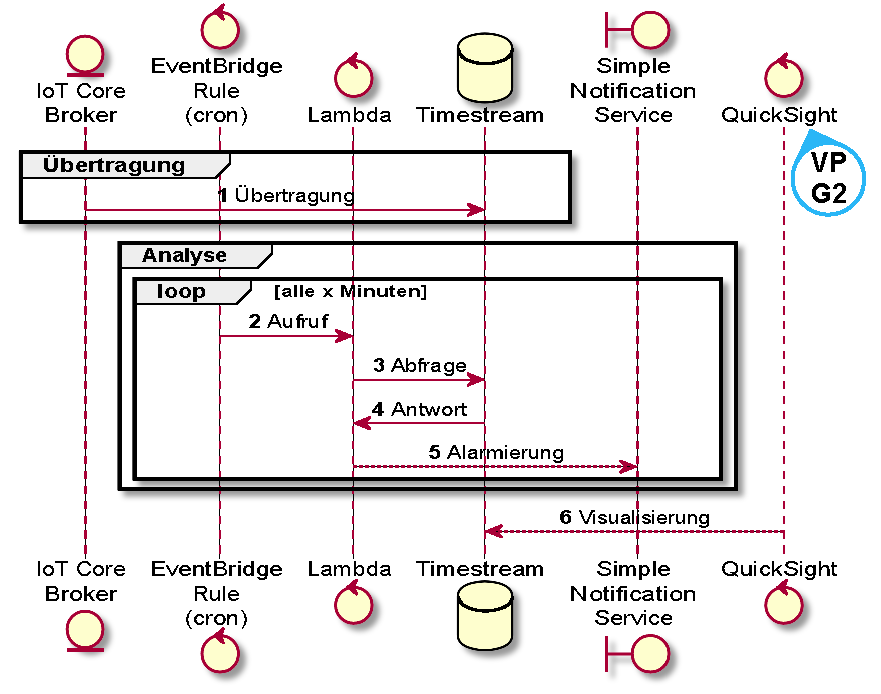
\includegraphics[height=0.38\textheight]{graphics/batch-ra.pdf}
\caption{Sequenzdiagramm Batch Verarbeitung}
\label{abb:SequenceBatchRA}
\end{figure}

\textbf{Variationspunkt G2:} Hier wird eine Dashboardinglösung, im speziellen der \ac{AWS} eigene Dienst QuickSight vorgesehen. Dies erfolgt, damit Benachrichtigungen, die via \ac{SNS} versendet werden, leicht für die Benachrichtigten nachvollziehbar sind. Wenn also beispielsweise eine Anomalie erkannt wurde, kann dies mit einer Visualisierung nachvollzogen werden, um dann entsprechend zu handeln. Wichtig ist, dass die Visualisierung sowohl von den Originaldaten aus dem Speicher von Timestream gespeist wird, als auch aus der Analyse. Das für und wieder des Einsatzes wurde auch bereits in \vpref{G2} der Echtzeitarchitektur diskutiert. Alternativ ist Timestream auch mit Grafana und damit dem Managed Service von Grafana integriert.\footcite[Vgl.][]{AmazonWebServicesInc..o.J.bm}\nzitat\footcite[Vgl.][]{Dutt.2020} Grafana kann dabei ebenfalls als Dashboardinglösung verwendet werden und kostet dabei das selbe wie die Standard Edition von QuickSight, nämlich 9\$ für Nutzende monatlich.\footcite[Vgl. auch im Foglenden][]{AmazonWebServicesInc..o.J.bn}\nzitat\footcite[Vgl.][]{AmazonWebServicesInc..o.J.bo} Erweiterte Kapazitäten bei QuickSight kosten 18\$ pro Monat für Nutzende. 



\subsection{Verteilungssicht}
In der folgenden \autoref{abb:TopLevelDBRA} ist die Verteilungssicht der Referenzarchitektur gemeinsam mit den Variationspunkten gezeigt. Variationspunkte mit Präfix G können dabei auch auf bereits definierte Variationspunkte der Echtzeitreferenzarchitektur referenzieren.
\begin{figure}[H]
\centering
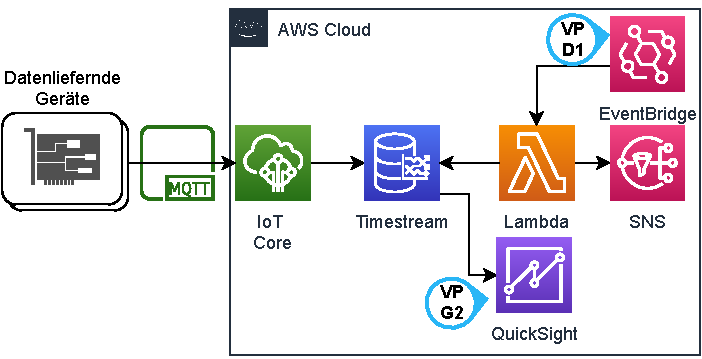
\includegraphics[width=\textwidth]{graphics/DB-RA-Overview.pdf}
\caption{Verteilungssicht}
\label{abb:TopLevelDBRA}
\end{figure}

\vp{D1}: EventBridge bietet den zeitlich geplanten Aufruf von Zielen wie Lambda an. Wenn keine kontinuierliche Überwachung gewünscht ist, kann die Lambda auch auf Bedarf ausgelöst werden. Dies wäre beispielsweise durch ein vorgelagertes API Gateway möglich. Über dieses muss dann der Zeitraum übergeben werden, für welchen die aktuelle Analyse durchgeführt werden soll.

\textbf{Variationspunkt G2:} Siehe Erläuterung in der Datenverarbeitungssequenz oder in \vpref{G2} der Echtzeitreferenzarchitektur.


\subsection{Bausteinsicht}
In der folgenden \autoref{abb:ElementeDBRA} wird die Bausteinsicht als tiefere Dekomposition der Verteilungssicht, samt Variationspunkten dargestellt.
\begin{figure}[H]
\centering
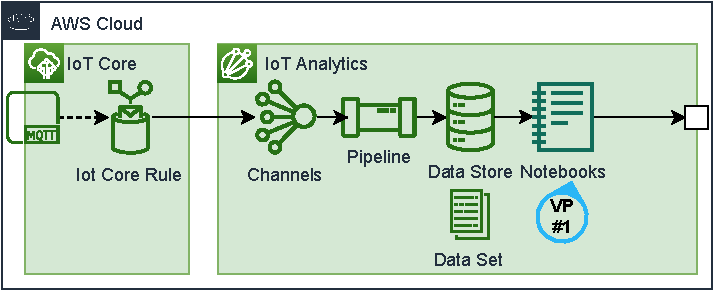
\includegraphics[width=\textwidth]{graphics/DB-RA-Elements.pdf}
\caption{Bausteinsicht}
\label{abb:ElementeDBRA}
\end{figure}

\vp{E1}: Timestream bietet aktuell zwei Speicherklassen an und hat eine Speicherklasse, die für die Zukunft angekündigt ist. Aktuell verfügbar sind \ac{RAM}-basierter Speicher, der teurer ist und magnetischer \ac{HDD}-Speicher, der günstiger ist. Mittels sogenannter \textit{retention policies} können Daten zwischen den Speicherklassen verschoben werden.\footcite[Vgl. auch im Folgenden][]{AmazonWebServicesInc..o.J.bp} Dabei können Daten vom \ac{RAM}-Speicher in den \ac{HDD}-Speicher verschoben werden und vom \ac{HDD}-Speicher gelöscht werden. Beim finalen Löschen der Daten sind die jeweiligen Anforderungen an Datenaufbewahrung der instanziierenden Architektur zu beachten. So können beispielsweise Langzeitanalysen notwendig sein, die auf einen Datenbestand von mehreren Monaten oder Jahren zugreifen müssen. Da Timestream aber auch nach Speicher abgerechnet wird, sind \textit{retention policies} sowohl von \ac{RAM} zu \ac{HDD} als auch zur Löschung von Inhalt vom \ac{HDD}-Speicher einzurichten. Zu beachten ist, dass die Gesamtaufbewahrungsdauer sich aus der Summe beider Aufbewahrungszeiten ergibt. Die Einstellung der \ac{RAM} zu \ac{HDD} retention policy ist abhängig von \vpref{E2} und \vpref{E5}, da je nach Abfragerhythmus und abgefragter Datenmenge für Analysen eine verlängerte Aufbewahrung im \ac{RAM} zur beschleunigten Analyse sinnvoll ist. Für die \ac{SQL}-Abfragen wird kein Unterschied zwischen Speicherart gemacht, bis auf die technisch bedingte höhere Ausführungsdauer auf \ac{HDD}-Speichern.

\vp{E2}: \ac{SQL}-Abfragen in Timestream sind auf mehrere Arten optimierbar. Zum einen wird die abgefragte Datenmenge in Rechnung gestellt, was eine präzise Einschränkung der Abfrage mit \mintinline[breaklines]{sql}{WHERE} Bedingungen und einem genauen \mintinline[breaklines]{sql}{SELECT} notwendig macht. Zusätzlich ist die Datenabfrage in zwei Modellen möglich: dem flachen Modell und dem Zeitreihenmodell. \footcite[Vgl. auch im Folgenden][]{AmazonWebServicesInc..o.J.bq} Das flache Modell schreibt, wie in \autoref{tab:flat-timestream} gezeigt, für jeden Messwert eine eigene Zeile. Entsprechend muss der Messwert in der \mintinline[breaklines]{sql}{WHERE} Bedingung spezifiziert werden.

\begin{table}[H]
\centering
\begin{tabular}{|l|l|l|l|l|}
\hline
time & \begin{tabular}[c]{@{}l@{}}Dimension A\\ (Sensorname)\end{tabular} & measure\_name & \begin{tabular}[c]{@{}l@{}}measure\_value\\ ::double\end{tabular} & \begin{tabular}[c]{@{}l@{}}measure\_value\\ ::bigint\end{tabular} \\ \hline
\begin{tabular}[c]{@{}l@{}}2021-05-10\\ 23:59:59\end{tabular} & sensora & co2 & null & 500 \\ \hline
\begin{tabular}[c]{@{}l@{}}2021-05-10\\ 23:59:59\end{tabular} & sensorb & temperature & 25.5 & null \\ \hline
\end{tabular}
\caption{Beispiel flaches Datenabrufmodell}
\label{tab:flat-timestream}
\end{table}

Gegensätzlich dazu gibt das Zeitreihenmodell, welches sich beispielsweise mit der \\ \mintinline[breaklines]{sql}{CREATE_TIME_SERIES} Funktion erzeugen lässt, \ac{JSON} Arrays zurück. Diese sehen wie folgt aus: \mintinline[breaklines]{json}{[{"time":"2021-05-10 23:59:59","value":500}]}. Timestream bietet für diese Zeitreihen spezielle Funktionen, wie beispielsweise die Interpolation fehlender Werte an.



\vp{E3}: Der Programmcode und die Laufzeit der Lambdafunktion in diesem Variationspunkt sind je nach Anforderungen und Kentnissen des Implementierungsteams bei der Instanziierung dieser Referenzarchitektur anzupassen/neu zu schreiben. In \anhangref{anhang:batch-codesample} ist beispielhaft eine Lambdafunktion, geschrieben in Javascript für die Node.js Laufzeitumgebung, gezeigt. Diese Lambdafunktion sendet eine \ac{SQL}-Abfrage zur Zählung von schwellwertüberschreitenden Werten einzelner Sensoren. Folgend werden die Ergebnisse ausgewertet und für jeden Sensor mit überschreitenden Messwerten eine Benachrichtigung via SNS und ein \textit{shutdown}-Befehl an den Sensor via \ac{MQTT} versendet. Zu beachten ist, dass Lambdafunktionen einen Timeout von 15 Minuten haben.\footcite[Vgl.][]{AmazonWebServicesInc..o.J.bv} 

Sollten besonders aufwändige Auswertungen durch die Lambdafunktion durchgeführt werden, sollte sie in ein Orchestrierungsdienst wie Step Functions eingebunden werden. Step Functions kann Aufgaben wie automatische Neuversuche oder Fortsetzung der Abfrage durch Übergabe der Abfrage-ID von Timestream erledigen. Ein möglicher Ablauf für StepFunctions ist in \autoref{abb:StepFunctionsRA} gezeigt. Dabei ist zu beachten, dass eine EventBridge Rule immernoch notwendig ist, die die StepFunction auslöst. Der vorgestellte Ablauf beruht auf der Annahme, dass der Code der Lambdafunktion vor Ende der erlaubten 15 Minuten sich selbst terminiert und die ID der aktuellen Abfrage an StepFunction zurückgibt. Die verbleibende Zeit ist für die Lambdafunktion mittels der \mintinline[breaklines]{javascript}{getRemainingTimeInMillis()} Methode (in der Node.js Laufzeitumgebung, andere können abweichen) transparent.\footcite[Vgl.][]{AmazonWebServicesInc..o.J.bw} Terminiert sich eine Lambdafunktion also mit der QueryID der noch laufenden Abfrage selber, wird ein erneuter Aufruf der Lambdafunktion mit der ID als Parameter von StepFunctions orchestriert. In dem dargestellten Ablauf übernimmt StepFunctions auch das Versenden der Alarme via \ac{SNS}. Dies ist nicht unbedingt notwendig und könnte auch weiter von der Lambdafunktion übernommen werden.

\begin{figure}[H]
\centering
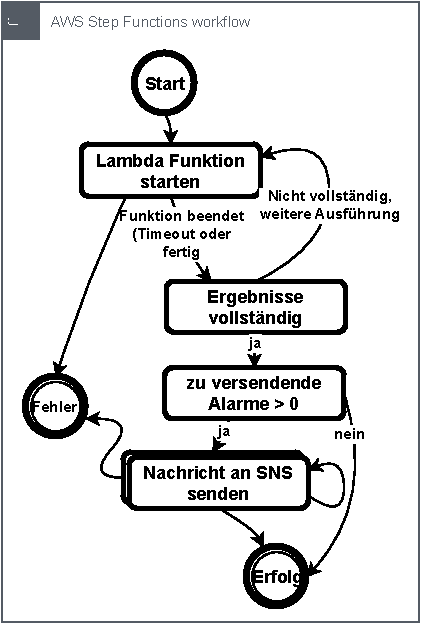
\includegraphics[height=0.45\textheight]{graphics/Zustaende-DB-RA.pdf}
\caption{Unformalisiertes Ablaufdiagramm StepFunctions}
\label{abb:StepFunctionsRA}
\end{figure}

\vp{E4}: Unabhängig von dem in \vpref{G2} gewählten Dienst ist es möglich, individuelle Dashboards mit unterschiedlichen Interaktionsmöglichkeiten zu erstellen. So können beispielsweise sogenannte \textit{drill-downs} den Nutzenden Entscheidungsträgern helfen, dynamisch die Datenbereiche anzupassen. Ein Dashboard in QuickSight kann beispielsweise wie folgt aussehen:
\begin{figure}[H]
\centering
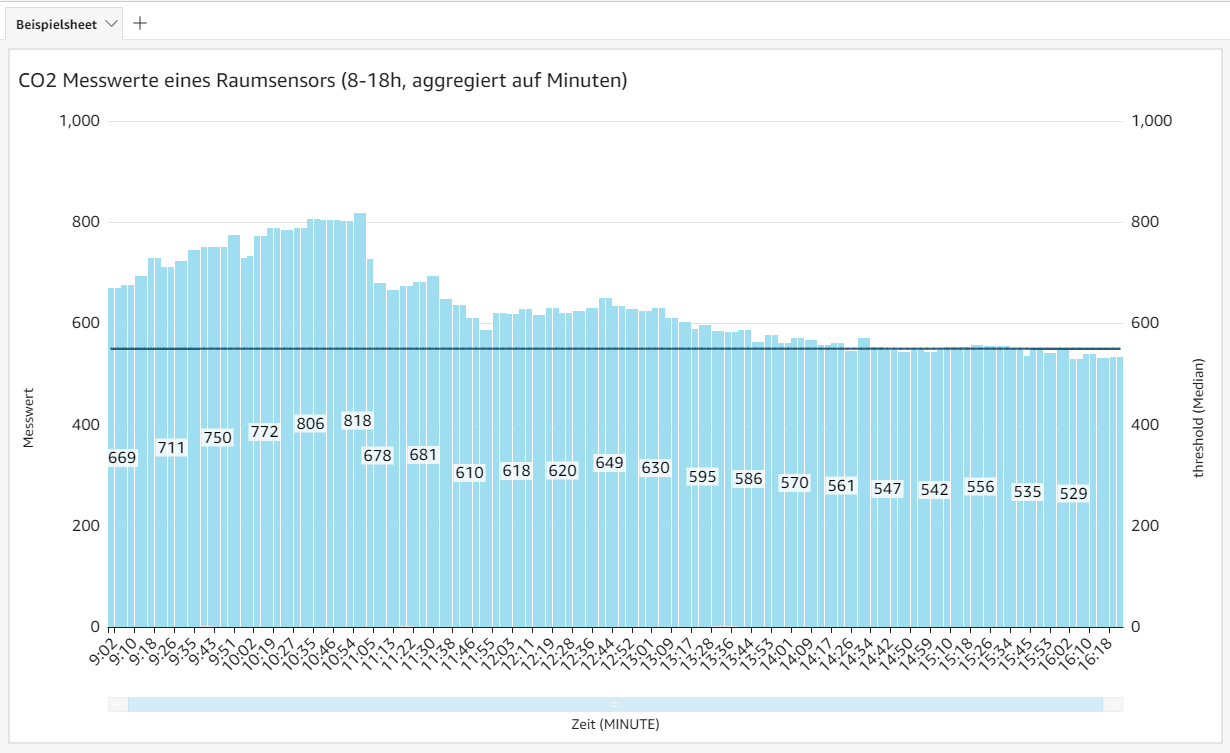
\includegraphics[width=\textwidth]{graphics/QuickSight-Beispiel.png}
\caption{Dashboard in QuickSight}
\label{abb:DashboardDBRA}
\end{figure}

\vp{E5}: EventBridge Regeln können unterschiedlich eingestellt werden. Abhängig von den Anforderungen der instanziierenden Architektur, kann entweder ein Aufruf alle x Minuten, Stunden oder Tage eingestellt werden, oder für mehr Anpassung eine Rate mittels einer abgewandelten, \textit{cron}-Syntax konfiguriert werden. Ein cron-Ausdruck, um die Regel alle 10 Minuten an Werktagen zwischen 9 und 17.00 Uhr auszulösen, sähe wie folgt aus: \mintinline[breaklines]{bash}{0/10 9-17 ? * MON-FRI *}. Der Ausdruck wird in \ac{UTC}-Zeit ausgeführt, was eine ein- oder zweistündige Verschiebung von der deutschen Zeit bedeutet.


\subsection{Anforderungen}
Folgend wird für die Batch Architektur dargestellt, wie die einzelnen Anforderungen mittels der Referenzarchitektur addressierbar sind.

\miniabschnitt{Anwendbarkeit auf Monitoringdaten (IT)}
Timestream unterstüzt wie die Kinesis Familie diverse Zeitreihendaten. Es ist ebenfalls prinzipiell möglich Logdaten aufzubewahren, da der interne Datentyp \textit{varchar} Strings mit bis zu 2 GB Länge erlaubt.\footcite[Vgl.][]{AmazonWebServicesInc..o.J.br} Da aber große Datenmengen in einzelnen Variablen durch die doppelten Kosten für Speicherung und Abfrage sich weniger eignen als beispielsweise numerische Messwerte, sollte auf die Anwendung auf Logs verzichtet werden.

Die Nutzung zur Speicherung von Metriken hingegen ist explizit im Rahmen von \textit{DevOps}-Anwendungsfällen für Timestream vorgesehen.\footcite[Vgl.][]{AmazonWebServicesInc..o.J.ak}\nzitat\footcite[Vgl.][]{Das.2020} Ohne spezialisierte Applikation, die beispielsweise in Kinesis Data Analytics mit Flink Laufzeitumgebung laufen könnte und von Kinesis Data Firehose gespeist wird, ist es jedoch nicht möglich CloudWatch Metriken in Timestream zu laden.\footcite[Vgl.][]{Riddle.2021} Alternativ können Metriken wie von \citeauthor{Pochiraju.2020} vorgeschlagen, über \ac{MQTT} und \AWSIOT{} Core in Timestream eingespeist werden.\footcite[Vgl.][]{Pochiraju.2020} Das eine eigene Applikation verwendet werden muss, um Daten via Kinesis oder \ac{MQTT} einzuspeisen, wertet die Tauglichkeit für Monitoring-Usecases gegenüber der Echtzeitarchitektur ab.


\miniabschnitt{Anwendbarkeit auf Sensordaten (IoT)}
Durch die native Integration mit \AWSIOT{} Core ist eine Integration mit Datensätzen von Sensoren, die via \ac{MQTT} übermittelt wurden vollständig verwaltet möglich. Metadaten der Sensoren können zur Attributierung bei der Auswertung mittels der Dimensionen übermittelt werden, Messwerte als eben solche. Die Menge an Erkenntnissen, die sich aus der Analyse der Sensordaten in Timestream gewinnen lassen, ist wesentlich von \vpref{E5} und damit der Analysefrequenz abhängig.

\miniabschnitt{Handling von Events, Messwerten und \enquote{Streaming}}
Timestream ist vollständig verwaltet und es sind keine Infrastrukturkomponenten zur Skalierung anzupassen. Da laut Aussage von \ac{AWS} mit dem Dienst Billionen Datenpunkte pro Tag nahe der Echtzeit verarbeitet und abgefragt werden können, ist zu erwarten, dass auch hochfrequente Datenreihen in angemessener Zeit gespeichert werden können.\footcite[Vgl.][]{AmazonWebServicesInc..2020g} Dabei wäre es, wenn die Dateneingangslogik selbst zu schreiben wäre möglich, dass wiederholbare Fehler auftreten. Da aber die Daten automatisiert nach dem Eingang im \ac{MQTT} Broker \AWSIOT{} Core in Timestream gespeichert werden, ist dies nicht nötig. Ein mögliches Problem gibt es maximal bei der Überttragungslatenz zwischen \AWSIOT{} Core und Timestream, auf die kein Einfluss genommen werden kann.
Da Timestream abseits der numerischen Datentypen auch Datentypen vie \textit{varchar} anbietet, ist es möglich auch Events in Timestream abzuspeichern.\footcite[Vgl.][]{AmazonWebServicesInc..o.J.r}


\miniabschnitt{Automatisierte operative Entscheidungen}
Das Codebeispiel in \anhangref{anhang:batch-codesample} demonstriert, dass es möglich ist, basierend auf den Ergebnissen einer Abfrage automatisiert Abfragen durchzuführen. Dabei zu beachten ist jedoch, dass durch die Intervallverzögerung Aktionen im schlechtesten Fall nach genau $t$ Minuten, nach dem Ereignis ausgelöst werden. Dabei ist $t$ das Intervall zwischen einzelnen Ausführungen, wie beschrieben in \vpref{E5}. Dies kann bei kritischen Aktionen, die möglichst schnell ausgeführt werden sollen jedoch die akzeptable Raktionszeit stark überschreiten. Sollte Timestream ähnlich zu Amazons DynamoDB integrierte Streams als Feature bekommen, welche Änderungen am Datensatz zur Verarbeitung an Plattformen wie Lambda senden, wäre dieses Problem addressierbar.

\subsection{Produktives Monitoringkonzept}
Um die Batch-Referenzarchitektur nach Instanziierung für einen Usecase möglichst störungsfrei betreiben zu können, sind folgend die zu überwachenden Metriken gelistet, die einen Fehler innerhalb des verteilten Systems anzeigen.\autoref{tab:cloudwatch-metrics-db} enthält die Cloud-Watch Metriken der Dienste TimeStream, Lambda, \ac{SNS}, \AWSIOT{} Core und EventBridge.\footcite[Vgl.][]{AmazonWebServicesInc..o.J.be}\nzitat\footcite[Vgl.][]{AmazonWebServicesInc..o.J.bf}\nzitat\footcite[Vgl.][]{AmazonWebServicesInc..o.J.bc}\nzitat\footcite[Vgl.][]{AmazonWebServicesInc..o.J.az}\nzitat\footcite[Vgl.][]{AmazonWebServicesInc..o.J.bl}


\begin{table}[H]
\centering
\begin{tabular}{|l|l|l|l|}
\hline
Dienst & Metrik & Ursache & Detektionsart \\ \hline
\rowcolor[HTML]{F5F5F5} 
\ac{SNS} & NumberOfNotificationsFailed & Dienstfehler & Schwellwert \\ \hline

\multirow{2}{*}{\AWSIOT{} Core} & RuleMessageThrottled & \begin{tabular}[c]{@{}l@{}}Dienstfehler/\\ Benutzungsfehler\end{tabular} & Schwellwert \\ \cline{2-4} 
 & Failure & \begin{tabular}[c]{@{}l@{}}Dienstfehler/\\ Benutzungsfehler\end{tabular} & Schwellwert \\ \hline
 
\rowcolor[HTML]{F5F5F5} 
\cellcolor[HTML]{F5F5F5} & SystemErrors & Dienstfehler & Schwellwert \\ \cline{2-4} 
\rowcolor[HTML]{F5F5F5} 
\cellcolor[HTML]{F5F5F5} & UserErrors & Benutzungsfehler & Schwellwert \\ \cline{2-4} 
\rowcolor[HTML]{F5F5F5} 
\multirow{-3}{*}{\cellcolor[HTML]{F5F5F5}TimeStream} & SuccessfulRequestLatency & \begin{tabular}[c]{@{}l@{}}Dienstfehler/\\ Benutzungsfehler\end{tabular} & Anomalie \\ \hline

\multirow{3}{*}{Lambda} & Duration & \begin{tabular}[c]{@{}l@{}}Dienstfehler/\\ Benutzungsfehler\end{tabular} & Anomalie \\ \cline{2-4} 
 & Errors & \begin{tabular}[c]{@{}l@{}}Dienstfehler/\\ Benutzungsfehler\end{tabular} & Schwellwert \\ \cline{2-4} 
 & Throttles & Benutzungsfehler & Schwellwert \\ \hline
 
\rowcolor[HTML]{F5F5F5} 
\cellcolor[HTML]{F5F5F5} & FailedInvocations & Dienstfehler & Anomalie \\ \cline{2-4} 
\rowcolor[HTML]{F5F5F5} 
\multirow{-2}{*}{EventBridge} & ThrottledRules & Dienstfehler & Schwellwert \\ \hline
\end{tabular}
\caption{CloudWatch Metriken}
\label{tab:cloudwatch-metrics-db}
\end{table}

\AWSIOT{} Core, \ac{SNS} und Timestream übermittelt Metriken in einminütiger Auflösung.\footcite[Vgl.][]{AmazonWebServicesInc..o.J.az}\nzitat\footcite[Vgl.][]{AmazonWebServicesInc..2021b}\nzitat\footcite[Vgl.][]{AmazonWebServicesInc..o.J.be} 
Bei Lambda können die übermittelten Metriken bis nach Ende einer Ausführung übermittelt werden, weshalb die Auflösung der Metriken unpräzise sein kann. Insgesamt lässt sich aufgrund der teilweise verketteten Metriken leicht erkennen, wenn kaskadierende Fehler auftreten. So sind beispielsweise \textit{FailedInvocations} von EventBridge ein Hinweis darauf, dass es Probleme bei der Ausführung von Lambda Funktionen gab.



\subsection{Know-how für instanziierende Architekturen}
Folgend werden die regionale Verfügbarkeit, die Datenstruktur und die Datenmodellierung für und von Timestream erläutert. Diese sind zu beachten bei der Instanziierung der Referenzarchitektur. 

\miniabschnitt{Regionale Verfügbarkeit}
Während Timestream zum Start 2020 allein in Irland (eu-west-1) für die EU verfügbar war, ist Timestream für die Region eu-central-1 (Frankfurt) mittlerweile verfügbar.\footcite[Vgl.][]{AmazonWebServicesInc..2020g}\nzitat\footcite[Vgl.][]{AmazonWebServicesInc..o.J.q} Dies erleichtert die Integration in bestehende Dienste, die bereits in Frankfurt provisioniert wurden.

\miniabschnitt{Datenstruktur}
Zeitreihen mit Messwerten und Metadaten werden innerhalb von Timestream als Dimensionen oder Messwerte hinterlegt. Dimensionen und Messwerte haben jeweils einen Namen und einen Wert. Dabei sind als Dimensionen alle Metadaten des übermittelnden Sensors oder der übermittelnden Applikation denkbar. Beispiele für solche Dimensionen wären Name oder Standort, während Messwerte beispielsweise \coo{} Messungen, Temperaturen, CPU Auslastung oder \ac{RAM}-Verbrauch sein können. Timestream rechnet pro Schreibzugriff die Summe aller Namen von Dimensionen und Messwerten und deren Werte (inklusive der Zeitdimension mit aktuellem Zeitstempel) als Speicherplatz ab.\footcite[Vgl. auch im Folgenden][]{AmazonWebServicesInc..o.J.bs} Bei gruppierten Schreibzugriffen können gemeinsame Attribute und Werte zusammengefasst werden, um die Anzahl an Schreibzugriffen zu vermindern.

\miniabschnitt{Datenmodellierung}
Aus der Unterteilung in Messwerte und Dimensionen ergeben sich auch Optimierungen der Datenmodellierung. So gibt es beispielsweise die Möglichkeit, derivative Werte, sofern sie eine niedrige Kardinalität besitzen als Dimensionen statt als Messwerte zu speichern.\footcite[Vgl. auch im Folgenden][]{AmazonWebServicesInc..o.J.bt} Dies bringt aber den Nachteil mit sich, dass entsprechend drei verschiedene Zeitreihen entstehen würden, was bei der Abfrage zu beachten ist. Da Dimensionsnamen ebenfalls Speicherplatz verbrauchen, sind die Namen entsprechend des Ockhams Rasiermesser zu gestalten und die einfachste und kürzeste Variante auszuwählen. Bei der Datenmodellierung ist auch zu beachten, dass Messwerte entsprechend ihres eigentlichen Datentyps gespeichert werden und keine unbeabsichtigte Konversion in z.B. das \textit{varchar} Format auftritt. Da Messwerte bei Erstanlage eines Messwertes in einer Tabelle fest mit einem Datentypen assoziiert werden, ist eine Neuanlage mit entsprechender Datenmigration notwendig um Fehler zu korrigieren.



